% arara: xelatex: { shell: true, interaction: nonstopmode } if changed('tex') || changed(toFile('fefudoc.cls'))
%arara: biber if changed('bib') || changed('bcf') || changed('bbl')
%arara: xelatex: { synctex: true, shell: true } if changed('aux')
% !TeX document-id = {2e2f2d46-ef9b-47ad-990b-8fdc6dcf34fb}
% !TeX program = xelatex
% !TeX encoding = UTF-8
% !TeX spellcheck = ru_RU
% !TeX TXS-program:compile=txs:///xelatex/[--shell-escape]|txs:///view-pdf
% !TeX TXS-program:bibliography = txs:///biber

% Тип документа:
\documentclass[labwork]{fefudoc}

\usepackage{mathtools, amsfonts, amssymb} %основные математикие операторы и шрифты
\usepackage{graphicx} %вставка рисунков из файлов
\usepackage{listings} %исходный код
\lstset{ %общие параметры расширения listings
	basicstyle=\ttfamily, %основной стиль текста кода
	keywordstyle=\bfseries, %стиль ключевых слов
	commentstyle=\itshape, %стиль комментариев
	showstringspaces=false, %не подчеркивать пробелы в строках
	frame=single, %обвести рамкой
	tabsize=2 %размер табуляционного сдвига
}
\usepackage{threeparttable}

\location{Владивосток}
\Institute{Политехнический институт (Школа)}
\Department{Департамент электроники, телекоммуникации и приборостроения}
\specialty{11.03.02} %коды специальностей приведены в Общероссийском классификаторе 009-2016,
                     % а также в файлах details/barchelorspecialties.def (бакалавры)
					 % и в details/masterspecialties.def (магистранты)
\profile{Системы радиосвязи и радиодоступа}
\discipline{Параллельное программирование}

%Автор:
\author{Б3121-11.03.02втц}{Сидоров Иван Петрович}
%Преподаватель:
\teacher{кандидат технических наук}{}{доцент департамента ЭТиП}{Чусов Андрей Александрович}

%Название работы
\title{Изучение программной среды \LaTeX{} для написания литературных работ}

\year=2024

\begin{document}
\frontpage
\tableofcontents

\section{Об авторе работы}
Я закончил школу №23 в 2003~г. с углубленным изучением физики и математики. Моими любимыми предметами были физика, математика, а также технология. С детства меня интересовали средства и методы автоматизации технических процессов, способы управления и передачи управляющих сигналов.

Также в свободное время я люблю заниматься созданием видео и музыкой. Поэтому я поступил на нашу специальность в надежде получить знания и умения использовать современные технологии и средства построения инфокоммуникационных систем, научиться думать рационально и самостоятельно принимать решения о том, как подходить к проблемам, возникающим в этих областях знаний.

В будущем я надеюсь работать по профессии в таких компаниях, как Ростелеком или МТС, или решать задачи проектирования сетей связи в условиях специальных требований к надежности, отказо- и помехоустойчивости, информационной безопасности.

\section{Теоретическое решение задачи}
\paragraph{Условие.} Доказать, что
\begin{equation}\label{условие}
\lim_{n \to \infty} \sqrt[n]{n} = 1.
\end{equation}
\paragraph{Решение.} Найдем экстремум функции \eqref{условие}:
$$
\frac{d}{dn} \sqrt[n]{n}
 = \frac{d}{dn} n^\frac{1}{n}
 = \frac{d}{dn} e^{\ln n \cdot \frac{1}{n}}
 = \frac{d}{dn} e^{\frac{\ln n}{n}}
 = \Big(\frac{1}{n \cdot n} - \frac{\ln n}{n^2}\Big) e^\frac{\ln n}{n}
 = \frac{1 - \ln n}{n^2}.
$$

Из этой производной видно, что если $\ln n > 1$, то функция $\sqrt[n]{n}$ постоянно убывает.

При этом ясно, что при $n \geq 1$
$$
\sqrt[n]{n} \geq \sqrt[n]{1} = 1,
$$
поскольку $\sqrt[n]{x}$ растет с $x$, т.~к. $$\frac{d}{dx}\sqrt[n]{x} = \frac{x^{\frac{1}{n} - 1}}{n} > 0$$ при $x > 0$.
Следовательно,
\begin{equation}\label{нижняя граница}
\lim_{n\to\infty}\sqrt[n]{n} \geq 1.
\end{equation}

Рассмотрим теперь функцию $(1 + x)^n$ для всех неотрицательных действительных $x$ (то есть $x \in \mathbb{R}_+$).

Разложение функции $f(x)$ в ряд Тейлора вокруг точки $a \in \mathbb{R}$ имеет вид
\begin{equation}\label{Тэйлор}
f(x) = \sum_{i = 0}^\infty \Big(\frac{d^i}{d x^i} f(x)\Big)\Big\vert_{x = a} \frac{(x - a)^i}{i!}.
\end{equation}

Вычислим производные функции
\begin{equation}\label{f(x)}
f(x) = (1 + x)^n
\end{equation}
относительно $x$ в точке $x=0$:
\begin{gather*}
\frac{d^0}{d x^0} (1 + x)^n\vert_{x = 0} = (1 + x)^n\vert_{x = 0} = 1, \\
\frac{d^1}{d x^1} (1 + x)^n\vert_{x = 0} = n \cdot (1 + x)^{n-1}\vert_{x = 0} = n, \\
\frac{d^2}{d x^2} (1 + x)^n\vert_{x = 0} = n \cdot (n - 1) \cdot (1 + x)^{n-2}\vert_{x = 0} = n \cdot (n - 1).
\end{gather*}

В общем случае
$$
\frac{d^i}{d x^i} (1 + x)^n\vert_{x = 0}
 = n \cdot (n - 1) \cdot \ldots \cdot \big(n - (i - 1)\big) \cdot (1 + x)^n \vert_{x = 0}
 = n^{\underline{i}} (1+x)^n
 = n^{\underline{i}},
$$
где $$n^{\underline{i}} = \frac{n!}{(n-i)!} = n \cdot \ldots \cdot (n - i + 1)$$ --- убывающий факториал.

Поэтому, подставляя \eqref{f(x)} и производные в \eqref{Тэйлор} при $a = 0$, имеем
$$
(1 + x)^n = \sum_{i=0}^\infty n^{\underline{i}} \frac{x^i}{i!}
 = \sum_{i=0}^\infty \frac{n!}{(n-i)!i!} \cdot x^i.
$$

Все элементы данной суммы неотрицательны, поскольку $x \geq 0$, поэтому любое эта сумма больше либо равна любому из её слагаемых.
В частности, это справедливо для слагаемого при $i = 2$:
$$
(1 + x)^n
 \geq n^{\underline{2}} \cdot x^2
 = \frac{n!}{(n-2)! \cdot 2!} \cdot x^2
 = \frac{n \cdot (n-1)}{2} x^2.
$$

Подставим сюда вместо $x$ значение $\sqrt{\frac{2}{n-1}}$.
Тогда
$$
(1 + x)^n = \Big(1 + \sqrt{\frac{2}{n-1}}\Big)^n
 \geq \frac{n \cdot (n-1)}{2} x^2
 = \frac{n \cdot (n-1)}{2} \frac{2}{n-1}
 = n.
$$

Но тогда
$$
\sqrt[n]{n} \leq (1 + x) = 1 + \sqrt{\frac{2}{n-1}}.
$$

Тогда с учётом \eqref{нижняя граница} имеем
$$
1 \leq \sqrt[n]{n} \leq \lim_{n\to\infty} 1 + \sqrt{\frac{2}{n-1}} = 1,
$$
поэтому
$$
\sqrt[n]{n} = 1.
$$

\section{Численный эксперимент}
В рамках лабораторной работы был выполнен численный эксперимент, свидетельствующий о справедливости решения.
Исходный код реализации эксперимента представлен на рис.~\ref{исходник}.

\begin{figure}
\centering
\begin{lstlisting}[language=Python]
import math

def root(n):
	return round(n**(1/n), 4)

N = 20
for n in range(1, N + 1, 1):
	print('\\hline')
	print(f'{n} & {root(n)} & {n + N} & {root(n + N)}' +
		f'& {n + 2 * N} & {root(n + 2 * N)}' +
		f'& {n + 3 * N} & {root(n + 3 * N)}' +
		f'& {n + 4 * N} & {root(n + 4 * N)} \\\\')

import numpy
import matplotlib.pyplot as plt

n = numpy.arange(1, 101)
plt.plot(n, n**(1/n))
plt.show()
\end{lstlisting}
\caption{Исходный код реализации эксперимента на языке Python}
\label{исходник}
\end{figure}

Численные результаты выполнения указанного кода представлены в таблице~\ref{таблица с результатами}.
\begin{table}
\centering
\begin{threeparttable}
\caption{Результаты эксперимента}
\label{таблица с результатами}
\begin{tabular}{cc|cc|cc|cc|cc}
\hline
$n$ & $\sqrt[n]{n}$ & $n$ & $\sqrt[n]{n}$ & $n$ & $\sqrt[n]{n}$ & $n$ & $\sqrt[n]{n}$ & $n$ & $\sqrt[n]{n}$ \\
\hline
1 & 1.0 & 21 & 1.156& 41 & 1.0948& 61 & 1.0697& 81 & 1.0558 \\
\hline
2 & 1.4142 & 22 & 1.1509& 42 & 1.0931& 62 & 1.0688& 82 & 1.0552 \\
\hline
3 & 1.4422 & 23 & 1.1461& 43 & 1.0914& 63 & 1.068& 83 & 1.0547 \\
\hline
4 & 1.4142 & 24 & 1.1416& 44 & 1.0898& 64 & 1.0671& 84 & 1.0542 \\
\hline
5 & 1.3797 & 25 & 1.1374& 45 & 1.0883& 65 & 1.0663& 85 & 1.0537 \\
\hline
6 & 1.348 & 26 & 1.1335& 46 & 1.0868& 66 & 1.0655& 86 & 1.0532 \\
\hline
7 & 1.3205 & 27 & 1.1298& 47 & 1.0854& 67 & 1.0648& 87 & 1.0527 \\
\hline
8 & 1.2968 & 28 & 1.1264& 48 & 1.084& 68 & 1.064& 88 & 1.0522 \\
\hline
9 & 1.2765 & 29 & 1.1231& 49 & 1.0827& 69 & 1.0633& 89 & 1.0517 \\
\hline
10 & 1.2589 & 30 & 1.12& 50 & 1.0814& 70 & 1.0626& 90 & 1.0513 \\
\hline
11 & 1.2436 & 31 & 1.1171& 51 & 1.0801& 71 & 1.0619& 91 & 1.0508 \\
\hline
12 & 1.2301 & 32 & 1.1144& 52 & 1.0789& 72 & 1.0612& 92 & 1.0504 \\
\hline
13 & 1.2181 & 33 & 1.1118& 53 & 1.0778& 73 & 1.0605& 93 & 1.0499 \\
\hline
14 & 1.2074 & 34 & 1.1093& 54 & 1.0767& 74 & 1.0599& 94 & 1.0495 \\
\hline
15 & 1.1979 & 35 & 1.1069& 55 & 1.0756& 75 & 1.0593& 95 & 1.0491 \\
\hline
16 & 1.1892 & 36 & 1.1047& 56 & 1.0745& 76 & 1.0586& 96 & 1.0487 \\
\hline
17 & 1.1814 & 37 & 1.1025& 57 & 1.0735& 77 & 1.058& 97 & 1.0483 \\
\hline
18 & 1.1742 & 38 & 1.1005& 58 & 1.0725& 78 & 1.0574& 98 & 1.0479 \\
\hline
19 & 1.1676 & 39 & 1.0985& 59 & 1.0716& 79 & 1.0569& 99 & 1.0475 \\
\hline
20 & 1.1616 & 40 & 1.0966& 60 & 1.0706& 80 & 1.0563& 100 & 1.0471 \\
\hline
\end{tabular}
\end{threeparttable}
\end{table}

В результате визуализации этих результатов получен график, представленный на рисунке~\ref{график}.
\begin{figure}
\centering
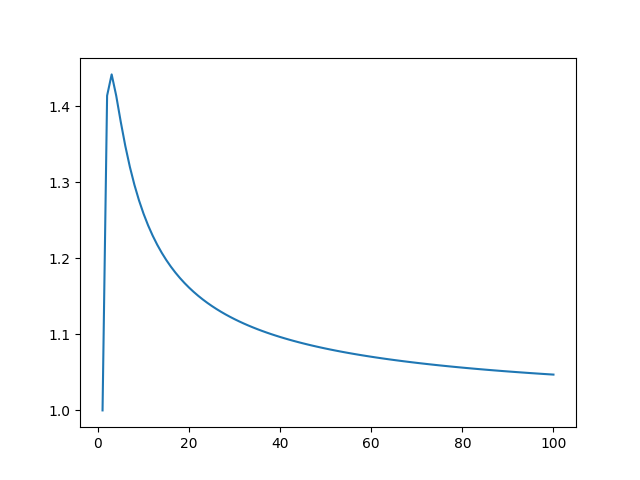
\includegraphics{labplot}
\caption{График функции $\sqrt[n]{n}$.}
\label{график}
\end{figure}

\section*{Заключение}
В результате работы мною были получены навыки\dots{} \textit{(написать самостоятельно)}

\end{document}

